\chapter{Problema 2}

\section{10362 - Trains}

Los trenes son fant�sticos. Puedes ir a donde quieras en tren, en europa, incluyendo pueblos peque�os. En Canada, el servicio de trenes no es muy bueno. A veces hay que cambiar de tren muchas veces y a menudo es dif�cil de saber cual es la ruta m�s r�pida, y donde realizar los cambios. Dependiendo de la hora del d�a, la ruta puede pasar por ciudades completamente diferentes. Afortunadamente, tu puedes escribir un programa para ayudar con esta tarea. Dados los horarios de los trenes recorriendo diferentes ciudades, tu tarea es encontrar todas las conexiones mas cortas entre dos lugares. Una conexi�n es mas corta que otra si no hay otra conexi�n que pueda dejarte salir mas tarde y llegar a la misma hora o mas temprano, o que saliendo al a misma hora llegue mas temprano o a la misma hora de llegada. Los tiempos de cambiar de tren no necesitan ser considerados, que se encuentran calculados dentro de los horarios.

\begin{figure}[H]
\centering
\label{ej2_trenes}
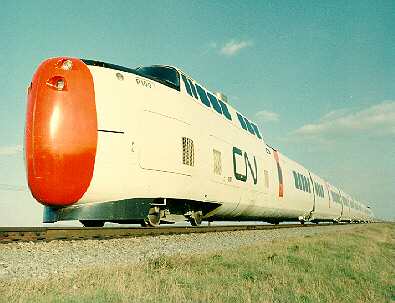
\includegraphics[scale=0.4]{./graficos/ej2/trains.jpg}
\end{figure}

\textbf{Entrada:}

La primer l�nea de entrada contiene un n�mero positivo $N$, que indica el n�mero de casos de test. La primer l�nea de cada caso de test contiene $T \le 20$ n�mero de l�neas de trenes. Cada l�nea de tren es descripta por una o mas l�neas conteniendo:

\begin{itemize}
\item El n�mero $S$ de estaciones en la l�nea de tren $S \le 20$, incluyendo el origen y el destino.
\item La hora de salida hh:mm del tren desde la primer estaci�n (en notaci�n de 24hs, es decir en el rango de  00:00 a 23:59). Se puede asumir que un tren deja la estaci�n de origen a la misma hora todos los d�as.
\item Una lista de nombres de las estaciones $S$, separadas por el tiempo de viaje entre las estaciones adyacentes. El tiempo de viaje es dado en horas y minutos.
\end{itemize}


Finalmente, cada caso de test da el nombre de una ciudad origen y destino para las cuales se tiene que armar un horario. Se puede asumir que hay al menos una ruta de la ciudad de origen hasta la ciudad destino.

\textbf{Salida:}

La salida consiste en una lista de las conexiones mas cortas desde el origen hasta el destino, indicando la hora de salida y el tiempo de viaje para cada una. Ordenadas por horario de salida. Cada horario de salida debe estar listado solo una vez si hay mas de una ruta con el mismo horario.

Los horarios de salida deben ser dados como $hh:mm$ (es decir exactamente 2 d�gitos en cado parte). El tiempo de viaje debe ser dado como $h:mm$, $hh:mm$, $hhh:mm$, etc. Se debe dejar una l�nea en blanco entre los resultados de cada caso de test.

\textbf{Url:}

\href{http://uva.onlinejudge.org/index.php?option=com_onlinejudge&Itemid=8&page=show_problem&category=15&problem=1303}{Problema de Trains}

\subsection{Modelo}

\subsection{Soluci�n}

\subsection{Detalles de implementaci�n}

\subsection{C�lculo de complejidad}